\documentclass{standalone}
% \documentclass{article}

\usepackage{tikz}

\begin{document}

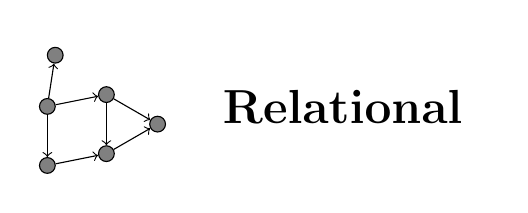
\begin{tikzpicture}
\draw[draw=none, fill=none] (0, 0) rectangle (6, 2);
\node at (4, 1) {\LARGE{\textbf{Relational}}};
\node (A) [style={minimum size=0.2cm,draw=black,fill=black!50,shape=circle,inner sep=0pt}] at (0.25, 0.25) {};
\node (B) [style={minimum size=0.2cm,draw=black,fill=black!50,shape=circle,inner sep=0pt}] at (0.25, 1.0) {};
\node (C) [style={minimum size=0.2cm,draw=black,fill=black!50,shape=circle,inner sep=0pt}] at (0.35, 1.65) {};
\node (D) [style={minimum size=0.2cm,draw=black,fill=black!50,shape=circle,inner sep=0pt}] at (1.0, 0.4) {};
\node (E) [style={minimum size=0.2cm,draw=black,fill=black!50,shape=circle,inner sep=0pt}] at (1.0, 1.15) {};
\node (F) [style={minimum size=0.2cm,draw=black,fill=black!50,shape=circle,inner sep=0pt}] at (1.65, 0.775) {};

\draw[->] (A) -- (D);
\draw[->] (B) -- (A);
\draw[->] (B) -- (C);
\draw[->] (B) -- (E);
\draw[->] (E) -- (D);
\draw[->] (E) -- (F);
\draw[->] (D) -- (F);
\end{tikzpicture}

\end{document}
